\documentclass{beamer}
%
% Choose how your presentation looks.
%
% For more themes, color themes and font themes, see:
% http://deic.uab.es/~iblanes/beamer_gallery/index_by_theme.html
%
\mode<presentation>
{
  \usetheme{default}      % or try Darmstadt, Madrid, Warsaw, ...
  \usecolortheme{default} % or try albatross, beaver, crane, ...
  \usefonttheme{default}  % or try serif, structurebold, ...
  \setbeamertemplate{navigation symbols}{}
  \setbeamertemplate{caption}[numbered]
  \setbeamertemplate{footline}[frame number]
  \setbeamertemplate{itemize items}[circle]
%   \setbeamertemplate{theorems}[numbered]
  \setbeamercolor*{structure}{bg=white,fg=blue}
  \setbeamerfont{block title}{size=\normalsize}
  \setbeamercolor{bibliography entry author}{fg=black}
  \setbeamercolor{bibliography entry title}{fg=black}
  \setbeamercolor{bibliography entry note}{fg=black}
}

% \newtheorem{proposition}[theorem]{Proposition}
% \theoremstyle{definition}
% \newtheorem{algorithm}[theorem]{Algorithm}
% \newtheorem{idea}[theorem]{Idea}

\usepackage[english]{babel}
\usepackage[utf8]{inputenc}
\usepackage[T1]{fontenc}
\usepackage{nicefrac}
% \usepackage{tabularx}
% \usepackage{makecell}
% \usepackage{amsmath,amsfonts,amsthm,amssymb,mathrsfs,bbm,mathtools}
% \usepackage{enumitem}
\usepackage{tikz}
% \usetikzlibrary{patterns}
% \usetikzlibrary{intersections}
% \usepackage{pgfplots}
% \usepgfplotslibrary{fillbetween}
% \usepgfplotslibrary{dateplot}
% \usepackage{pgfplotstable}

% \usepackage{booktabs}
% \usepackage[final]{microtype}
% \usepackage{caption}
% \usepackage{amsmath}
% \usepackage{mathtools}
% \usepackage{amsthm,thmtools}
% % \usepackage[nottoc]{tocbibind}
% % \usepackage[ruled]{algorithm2e}
% \usepackage{enumerate}
% \usepackage[italic]{esdiff}
% \usepackage{subcaption}
% \usepackage{ltablex}
% \usepackage{multirow}

%--------Pseudocode--------
\usepackage{xcolor,amsmath}
\usepackage{algorithm2e}
\DontPrintSemicolon
% \SetAlgoSkip{bigskip}

% % Define pseudocode formatting
% \renewcommand{\KwSty}[1]{\textnormal{\textcolor{blue!90!black}{\ttfamily\bfseries #1}}\unskip}
% \renewcommand{\ArgSty}[1]{\textnormal{\ttfamily #1}\unskip}
% \SetKwComment{Comment}{\color{green!50!black}// }{}
% \renewcommand{\CommentSty}[1]{\textnormal{\ttfamily\color{green!50!black}#1}\unskip}
% \newcommand{\assign}{\leftarrow}
% % \newcommand{\var}{\texttt}
% \newcommand{\FuncCall}[2]{\texttt{\bfseries #1(#2)}}
% \SetKwProg{Function}{function}{}{}
% \renewcommand{\ProgSty}[1]{\texttt{\bfseries #1}}

% % Settings for pgfplots
% \pgfplotsset{compat=newest}

% \renewcommand\tabularxcolumn[1]{m{#1}}
% \newcolumntype{R}{>{\raggedleft\arraybackslash}X}=

% \def\code#1{\texttt{\frenchspacing#1}}
\def\padding{\vspace{0.5cm}}
\def\spadding{\vspace{0.25cm}}
\def\b{\textcolor{blue}}
\def\r{\textcolor{red}}
\def\g#1{{\usebeamercolor[fg]{block title example}{#1}}}

% % fix for \pause in align
% \makeatletter
% \let\save@measuring@true\measuring@true
% \def\measuring@true{%
%   \save@measuring@trueoread{##1}}{}}%
%   \def\beamer@sortzeroread##1<##2>{}%
%   \def\beamer@finalnospec{}%
% }
% \makeatother

% \DeclarePairedDelimiter{\norm}{\lVert}{\rVert}
\NewDocumentCommand{\follows}{}{\ensuremath{\rightsquigarrow}\hspace{0.5em}}
\newcommand*{\defeq}{\overset{.}{=}}
\newcommand*{\eqdef}{\overset{.}{=}}
\RenewDocumentCommand{\Pr}{om}{Pr\IfValueT{#1}{_{#1}}{}[#2]}
\NewDocumentCommand{\E}{om}{\mathbb{E}\IfValueT{#1}{_{#1}}{}#2}
\RenewDocumentCommand{\O}{m}{\mathcal{O}(#1)}
\NewDocumentCommand{\B}{}{\mathcal{B}}
\NewDocumentCommand{\G}{}{\mathcal{G}}
\NewDocumentCommand{\pmax}{}{p_\mathrm{max}}
\NewDocumentCommand{\var}{m}{\mathrm{var}(#1)}
\NewDocumentCommand{\compat}{mm}{#1/#2}

\usepackage[sorting=ynt,style=alphabetic]{biblatex}
\addbibresource{sources.bib}

\renewcommand{\footnotesize}{\tiny}

\begin{document}

\title[Deterministic Algorithms for the Lovász Local Lemma]{Deterministic Algorithms \\ for the Lovász Local Lemma\footfullcite{harris2022deterministic}}
\author{Jonas Hübotter and Duri Janett \\ Advised by Yassir Akram}
\date{March 29, 2022}

\begin{frame}
  \titlepage
\end{frame}

% \begin{frame}{Outline}
%  \tableofcontents[subsubsectionstyle=hide,pausesections]
% \end{frame}
% \AtBeginSection[]
%   {
%      \begin{frame}[allowframebreaks]{Plan}
%      \tableofcontents[currentsection, sectionstyle=show/hide, hideothersubsections]
%      \end{frame}
%   }

\section{Introduction}
\subsection{Lovász Local Lemma and the MT Algorithm}
\begin{frame}{Setting}
Distribution $\Omega$ over independent $\Sigma$-valued coordinates $X_1, \dots, X_n$.
``Bad-events'' $\B = \{B_1, \dots, B_m\}$, each a boolean function of some subset of coordinates $\var{B_i} \subseteq [n]$.\pause

\begin{example}[3-SAT]
\begin{columns}
\begin{column}{.3\textwidth}
$\begin{aligned}
B_1 &\defeq f_1(X_1,X_5,X_8) \\
B_2 &\defeq f_2(X_2,X_5,X_{10}) \\
B_3 &\defeq f_3(X_1,X_8,X_{10}) \\
B_4 &\defeq f_4(X_2,X_6,X_{11})
\end{aligned}$
\end{column}
\begin{column}{.3\textwidth}
\tikzset{every picture/.style={line width=0.75pt}} %set default line width to 0.75pt        

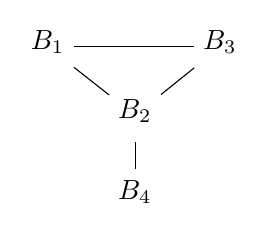
\begin{tikzpicture}[x=0.75pt,y=0.75pt,yscale=-1,xscale=1]
%uncomment if require: \path (0,534); %set diagram left start at 0, and has height of 534


% Text Node
\draw (20,22) node [anchor=north west][inner sep=0.75pt]    {$B_{1}$};
% Text Node
\draw (62,55) node [anchor=north west][inner sep=0.75pt]    {$B_{2}$};
% Text Node
\draw (103,22) node [anchor=north west][inner sep=0.75pt]    {$B_{3}$};
% Text Node
\draw (62,94) node [anchor=north west][inner sep=0.75pt]    {$B_{4}$};
% Connection
\draw    (100,31) -- (42,31) ;
% Connection
\draw    (59,54.18) -- (42,40.82) ;
% Connection
\draw    (84,53.94) -- (100,41.06) ;
% Connection
\draw    (71.5,77) -- (71.5,90) ;

\end{tikzpicture}
\end{column}
\end{columns}
\end{example}\pause

\begin{theorem}[(Symmetric) Lovász Local Lemma]
If for any $i$, $\Pr{B_i} \leq \pmax$ and $B_i$ affects at most $d$ bad-events, then $e \pmax d \leq 1$ implies $\Pr{\text{all $B_i$ avoided}} > 0$.
\end{theorem}\pause\spadding

For \g{$k$-SAT}, $p=2^{-k}$ \follows satisfiable if any literal appears in at most $d = \nicefrac{2^k}{e}$ clauses!\pause\ How to find a satisfying assignment?
\end{frame}

\begin{frame}{Prior Work}
\begin{algorithm}[H]
    \TitleOfAlgo{MT-Algorithm}
    Draw $X$ from distribution $\Omega$\;
    \While{some bad-event is true on $X$}{
        Select any true bad-event $B$\;
        For each $i \in \var{B}$, draw $X_i$ from its distribution in $\Omega$\;
    }
\end{algorithm}\pause
\follows converges within $\O{m}$ iterations in expectation.\footfullcite{moser2010constructive}\pause\spadding

What about deterministic algorithms?\pause\par
Polynomial-time algorithm if $e \pmax d \leq 1$ for any constant $\epsilon > 0$.\footfullcite{chandrasekaran2013deterministic}
\end{frame}

\subsection{Overview of Results}
\begin{frame}{Contributions}
\begin{enumerate}
    \item \emph{Deterministic algorithm} with a simpler \& weaker condition that is satisfied by \emph{most} variants of the LLL.\pause
    \item Faster \emph{parallel algorithm} with simpler conditions.\pause
    \item Algorithm that finds a configuration avoiding bad events such that the (weighted) probability of some auxiliary events is not much more than their expectation.
\end{enumerate}
\end{frame}

\section{Background}
\subsection{Alternative Characterization of MT Algorithm}
\begin{frame}{Plan}
\tableofcontents[currentsection, sectionstyle=show/shaded, hideothersubsections]
\end{frame}

\begin{frame}{Alternative Characterization of MT Algorithm}
Consider the \b{resampling table} $R$ drawn according to distribution $\Omega$:\spadding

\begin{columns}
\begin{column}{.2\textwidth}



\tikzset{every picture/.style={line width=0.75pt}} %set default line width to 0.75pt        

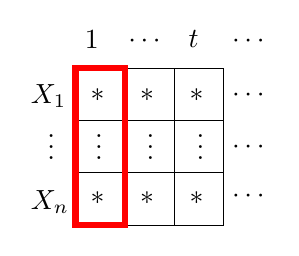
\begin{tikzpicture}[x=0.75pt,y=0.75pt,yscale=-1,xscale=1]
%uncomment if require: \path (0,534); %set diagram left start at 0, and has height of 534

%Shape: Rectangle [id:dp17271303952502315] 
% \draw   (52.81,325.2) -- (76.62,325.2) -- (76.62,350.41) -- (52.81,350.41) -- cycle ;
%Shape: Rectangle [id:dp4366577772656428] 
\draw   (76.81,350.41) -- (100.62,350.41) -- (100.62,375.62) -- (76.81,375.62) -- cycle ;
%Shape: Rectangle [id:dp13823281826780653] 
\draw   (76.81,325.2) -- (100.62,325.2) -- (100.62,350.41) -- (76.81,350.41) -- cycle ;
%Shape: Rectangle [id:dp25508926192152326] 
\draw   (100.62,325.2) -- (124.43,325.2) -- (124.43,350.41) -- (100.62,350.41) -- cycle ;
%Shape: Rectangle [id:dp7615695748694848] 
\draw   (124.43,325.2) -- (148.24,325.2) -- (148.24,350.41) -- (124.43,350.41) -- cycle ;
%Shape: Rectangle [id:dp7082057113045306] 
\draw   (100.62,350.41) -- (124.43,350.41) -- (124.43,375.62) -- (100.62,375.62) -- cycle ;
%Shape: Rectangle [id:dp5459336420864682] 
\draw   (124.43,350.41) -- (148.24,350.41) -- (148.24,375.62) -- (124.43,375.62) -- cycle ;
%Shape: Rectangle [id:dp8229762223203931] 
\draw   (76.81,375.62) -- (100.62,375.62) -- (100.62,400.83) -- (76.81,400.83) -- cycle ;
%Shape: Rectangle [id:dp7425833826219033] 
\draw   (100.62,375.62) -- (124.43,375.62) -- (124.43,400.83) -- (100.62,400.83) -- cycle ;
%Shape: Rectangle [id:dp11427372040336436] 
\draw   (124.43,375.62) -- (148.24,375.62) -- (148.24,400.83) -- (124.43,400.83) -- cycle ;
%Shape: Rectangle [id:dp835448558688529] 
\onslide<2->{\draw  [color={rgb, 255:red, 255; green, 0; blue, 0 }  ,draw opacity=1 ][line width=2.25]  (76.81,325.2) -- (100.62,325.2) -- (100.62,400.83) -- (76.81,400.83) -- cycle ;}

% Text Node
\draw (82.82,334.01) node [anchor=north west][inner sep=0.75pt]    {$*$};
% Text Node
\draw (106.63,334.01) node [anchor=north west][inner sep=0.75pt]    {$*$};
% Text Node
\draw (130.44,334.01) node [anchor=north west][inner sep=0.75pt]    {$*$};
% Text Node
\draw (82.82,383.43) node [anchor=north west][inner sep=0.75pt]    {$*$};
% Text Node
\draw (106.63,383.43) node [anchor=north west][inner sep=0.75pt]    {$*$};
% Text Node
\draw (130.44,383.43) node [anchor=north west][inner sep=0.75pt]    {$*$};
% Text Node
\draw (62,348) node [anchor=north west][inner sep=0.75pt]    {$\vdots $};
% Text Node
\draw (54,332) node [anchor=north west][inner sep=0.75pt]    {$X_1$};
% Text Node
\draw (54,383) node [anchor=north west][inner sep=0.75pt]    {$X_n$};
% Text Node
\draw (85,348) node [anchor=north west][inner sep=0.75pt]    {$\vdots $};
% Text Node
\draw (109.81,348) node [anchor=north west][inner sep=0.75pt]    {$\vdots $};
% Text Node
\draw (133.81,348) node [anchor=north west][inner sep=0.75pt]    {$\vdots $};
% Text Node
\draw (80,306) node [anchor=north west][inner sep=0.75pt]    {$1$};
% Text Node
\draw (101,308) node [anchor=north west][inner sep=0.75pt]    {$\cdots $};
% Text Node
\draw (130,306) node [anchor=north west][inner sep=0.75pt]    {$t$};
% Text Node
\draw (151,308) node [anchor=north west][inner sep=0.75pt]    {$\cdots $};
% Text Node
\draw (151,334) node [anchor=north west][inner sep=0.75pt]    {$\cdots $};
% Text Node
\draw (151,359) node [anchor=north west][inner sep=0.75pt]    {$\cdots $};
% Text Node
\draw (151,383) node [anchor=north west][inner sep=0.75pt]    {$\cdots $};
% Text Node
% \draw (57.82,334.01) node [anchor=north west][inner sep=0.75pt]    {$*$};


\end{tikzpicture}
\pause
\end{column}\pause
\begin{column}{.2\textwidth}
\flushright $\overset{\text{resampling $X_1$}}{\follows}$
\end{column}
\begin{column}{.3\textwidth}
\hspace{-2em}\input{figures/shifted_resampling_table}
\end{column}
\end{columns}\pause

When resampling $B_i$, shift rows $\var{B_i}$ to left.\pause\padding

\follows MT algorithm deterministic with respect to resampling table!
\end{frame}

\subsection{Outline}
\begin{frame}{Outline}
    Goal: Find a resampling table such that after poly. resamples all bad-events are avoided.\spadding
    
    Idea: Choose $R$ such that the MT algorithm only performs resamples that the randomized variant is likely to perform.\pause\padding
    
    \begin{enumerate}
        \item Construct set of unlikely resamples of randomized MT algorithm.\pause
        \item Use method of conditional expectations to find a resampling table $R$ such that all of these resamplings are avoided.\pause
        \item Simulate MT algorithm using $R$.
    \end{enumerate}
\end{frame}

\subsection{Counting Resamples}
\begin{frame}{Counting Resamples}
Find an injective mapping from resamples to some ``countable'' structure.\pause

\begin{block}{Mapping from executions}
Note: Given a resampling table $R$, a \b{(partial) execution} of the MT algorithm is described by the sequence of resampled bad-events.\spadding

\begin{columns}
\begin{column}{.15\textwidth}
\centering $B_1, B_2, B_3\onslide<4->{, \r{B_4}}$
\end{column}
\begin{column}{.05\textwidth}
\centering $\mapsto$
\end{column}\pause
\begin{column}{.2\textwidth}
\centering\only<-3>{


\tikzset{every picture/.style={line width=0.75pt}} %set default line width to 0.75pt        

\hspace{-1.3em}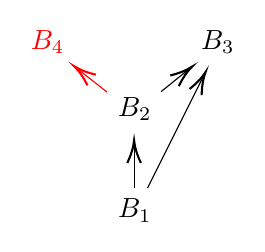
\begin{tikzpicture}[x=0.75pt,y=0.75pt,yscale=-1,xscale=1]
%uncomment if require: \path (0,534); %set diagram left start at 0, and has height of 534


% Text Node
\onslide<5->{\draw (241,27) node [anchor=north west][inner sep=0.75pt]  [color={rgb, 255:red, 255; green, 0; blue, 0 }  ,opacity=1 ]    {$B_{4}$};}
% Text Node
\draw (283,59) node [anchor=north west][inner sep=0.75pt]    {$B_{2}$};
% Text Node
\draw (323,27) node [anchor=north west][inner sep=0.75pt]    {$B_{3}$};
% Text Node
\draw (283,108) node [anchor=north west][inner sep=0.75pt]    {$B_{1}$};
% Connection
\onslide<5->{\draw [color={rgb, 255:red, 255; green, 0; blue, 0 }  ,draw opacity=1 ]    (279,57.79) -- (264.57,46.45) ;
\draw [shift={(263,45.21)}, rotate = 38.16] [color={rgb, 255:red, 255; green, 0; blue, 0 }  ][line width=0.75]    (10.93,-3.29) .. controls (6.95,-1.4) and (3.31,-0.3) .. (0,0) .. controls (3.31,0.3) and (6.95,1.4) .. (10.93,3.29)   ;}
% Connection
\draw    (305,57.54) -- (318.44,46.72) ;
\draw [shift={(320,45.46)}, rotate = 141.17] [color={rgb, 255:red, 0; green, 0; blue, 0 }  ][line width=0.75]    (10.93,-3.29) .. controls (6.95,-1.4) and (3.31,-0.3) .. (0,0) .. controls (3.31,0.3) and (6.95,1.4) .. (10.93,3.29)   ;
% Connection
\draw    (292,83) -- (292,104) ;
\draw [shift={(292,81)}, rotate = 90] [color={rgb, 255:red, 0; green, 0; blue, 0 }  ][line width=0.75]    (10.93,-3.29) .. controls (6.95,-1.4) and (3.31,-0.3) .. (0,0) .. controls (3.31,0.3) and (6.95,1.4) .. (10.93,3.29)   ;
% Connection
\draw    (298.5,104) -- (325.61,49.79) ;
\draw [shift={(326.5,48)}, rotate = 116.57] [color={rgb, 255:red, 0; green, 0; blue, 0 }  ][line width=0.75]    (10.93,-3.29) .. controls (6.95,-1.4) and (3.31,-0.3) .. (0,0) .. controls (3.31,0.3) and (6.95,1.4) .. (10.93,3.29)   ;

\end{tikzpicture}
}\only<4->{\input{figures/witness_dag_extended}}
\end{column}
\begin{column}{.4\textwidth}
\b{Witness DAG} $\hat{G}$

$B_i \longrightarrow B_j$ iff $i < j$ and $B_i$ affects $B_j$
\end{column}
\end{columns}\pause\pause

\follows $\hat{G}$ is always a DAG!
\end{block}
\end{frame}

\begin{frame}{Counting Resamples}
\begin{block}{Mapping from resamples}
\begin{columns}
\begin{column}{.15\textwidth}
resampling of $B_4$
\end{column}
\begin{column}{.05\textwidth}
\centering $\mapsto$
\end{column}
\begin{column}{.2\textwidth}
\centering\input{figures/witness_dag_subgraph}
\end{column}
\begin{column}{.1\textwidth}
\end{column}
\end{columns}\pause

Observe: Given a resampling table and $\hat{G}(B_i)$, we can uniquely reconstruct the values of $\var{B_i}$ before \& after resampling $B_i$.\pause\par
\follows the mapping is injective!\pause\spadding

% Also: The reconstructed configuration at step $i$ is sampled according to $\Omega$.
\end{block}
\end{frame}

\begin{frame}{Counting Resamples}
Do we map resamples to \emph{all} witness DAGs?\pause\par
No! \follows we can improve our counting!\pause\spadding

\begin{itemize}
    \item $\hat{G}(B_i)$ always has a single sink (set denoted $\G$)\pause
    \item Given resampling table $R$, not all single-sink witness DAGs $G$ correspond to a possible resample!\pause
    
    % TODO
    
    \follows $G$ \& $R$ must be \b{compatible} \pause(denoted $\Phi(G, R)$, set $\compat{\G}{R}$)\pause\spadding
    
    Note: $\Pr[R\sim\Omega]{\Phi(G,R)} \pause= \prod_{B \in G} \Pr{B} \pause\eqdef w(G)$.
\end{itemize}\pause\spadding

\follows for fixed resampling table $R$, at most $|\compat{\G}{R}|$ resamplings\pause\padding

$\E{|\compat{\G}{R}|} \pause= \sum_{G \in \G} \Pr{\Phi(G,R)} \pause= \sum_{G\in\G} w(G) \eqdef \underbrace{w(\G) \pause < \infty}_{\text{\b{Shearer Criterion}}}$.
\end{frame}

% \subsection{Counting Resamples with Witness DAGs}
% \subsubsection{What are Witness DAGs?}
% \begin{frame}{Frame Title}
    
% \end{frame}
% \subsubsection{From Witness DAGs to the Resampling Table to the MT Algorithm}
% \begin{frame}{Frame Title}
    
% \end{frame}
% \subsection{Shearer's Criterion}
% \begin{frame}{Frame Title}
    
% \end{frame}

% \section{A Deterministic Algorithm}
% \begin{frame}{Plan}
% \tableofcontents[currentsection, sectionstyle=show/shaded, hideothersubsections]
% \end{frame}
% \subsection{Shearer's Criterion with Slack}
% \begin{frame}{Frame Title}
    
% \end{frame}
% \subsection{Counting Witness DAGs}
% \begin{frame}{Frame Title}
    
% \end{frame}
% \subsection{Analyzing the Deterministic Algorithm}
% \begin{frame}{Frame Title}
    
% \end{frame}
% \subsection{Pre-processing the Witness DAG and Crisper Results}
% \begin{frame}{Frame Title}
    
% \end{frame}

% \section{Outlook: A Parallel Algorithm and the MT-distribution}
% \begin{frame}{Plan}
% \tableofcontents[currentsection, sectionstyle=show/shaded, hideothersubsections]
% \end{frame}
% \begin{frame}{Frame Title}
    
% \end{frame}

% \begin{frame}{}
%     \centering \large
%     Thanks for your attention!
%     Questions?
% \end{frame}

\end{document}